\chapter{日本地区机器学习方法预估震级效果}
\section{数据分析与预处理}
\indent 利用第二、三章所描述的方法,本文搭建并实现了$\tau_{c}$方法和机器学习类模型进行效果检验。考虑到震级紧急预估的应用场景和所需要的基础设施需求,我们将研究区域定位日本主岛区域附近。考虑到地震紧急预估的时效性,选取地震事件距离台站为1个相对经纬距离(约100km)内的记录。原始全数据集使用了日本KiK和KNET两台站网从2015至2017年所记录到的所有大于3级且震源靠近日本岛主体的地震记录,除此之外并无经过其他任何的主动事件挑选,事件分布如下图4.1所示。\\
\begin{figure}[!h]%%图
	\centering  %插入的图片居中表示
	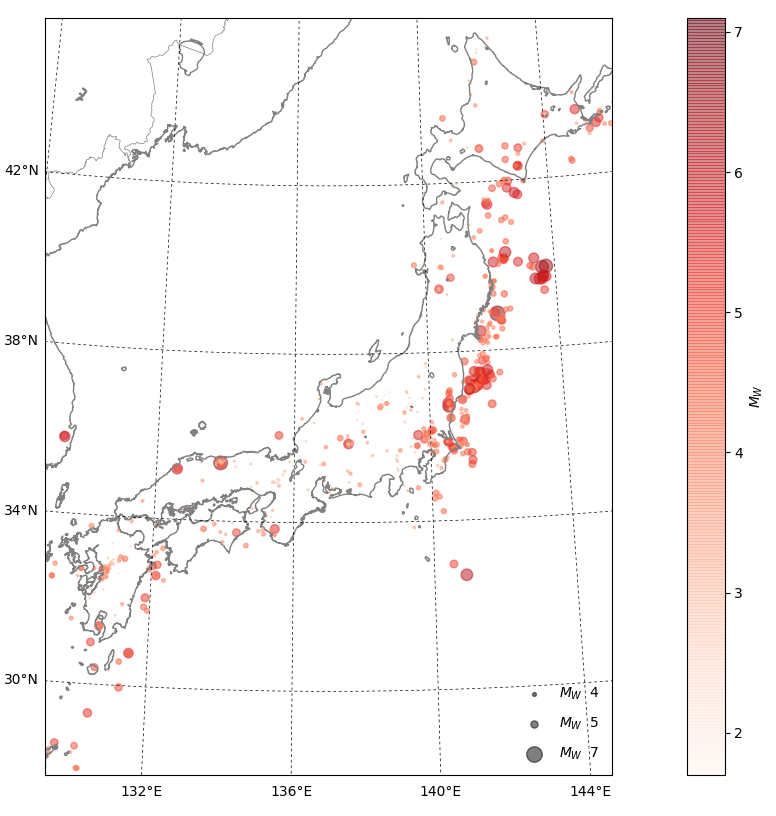
\includegraphics[width=\linewidth]{img/basemap.png}  %插入的图,包括JPG,PNG,PDF,EPS等,放在源文件目录下
	\caption{日本地区全数据集地震事件分布示意图}  %图片的名称
	\label{fig:mcmthesis-logo}   %标签,用作引用
\end{figure}
\indent 原始全数据中共包含了840个地震事件,合计50314条记录,具体的分布和统计如下图4.2和4.3所示,其中包含了3级至4级地震事件共420个、10145条地震台站记录,4级至5级地震事件共216个、14629条地震台站记录,5级至6级地震事件共61个、10740条地震台站记录,6级以上地震事件共8个、1004条地震台站记录。地震事件的分布特点如图4.2(b)所示存在很严重左偏,这种不均分布特征对机器学习模型训练带来一些阻碍。\\
\begin{figure}[!h]%%图
	\centering  %插入的图片居中表示
	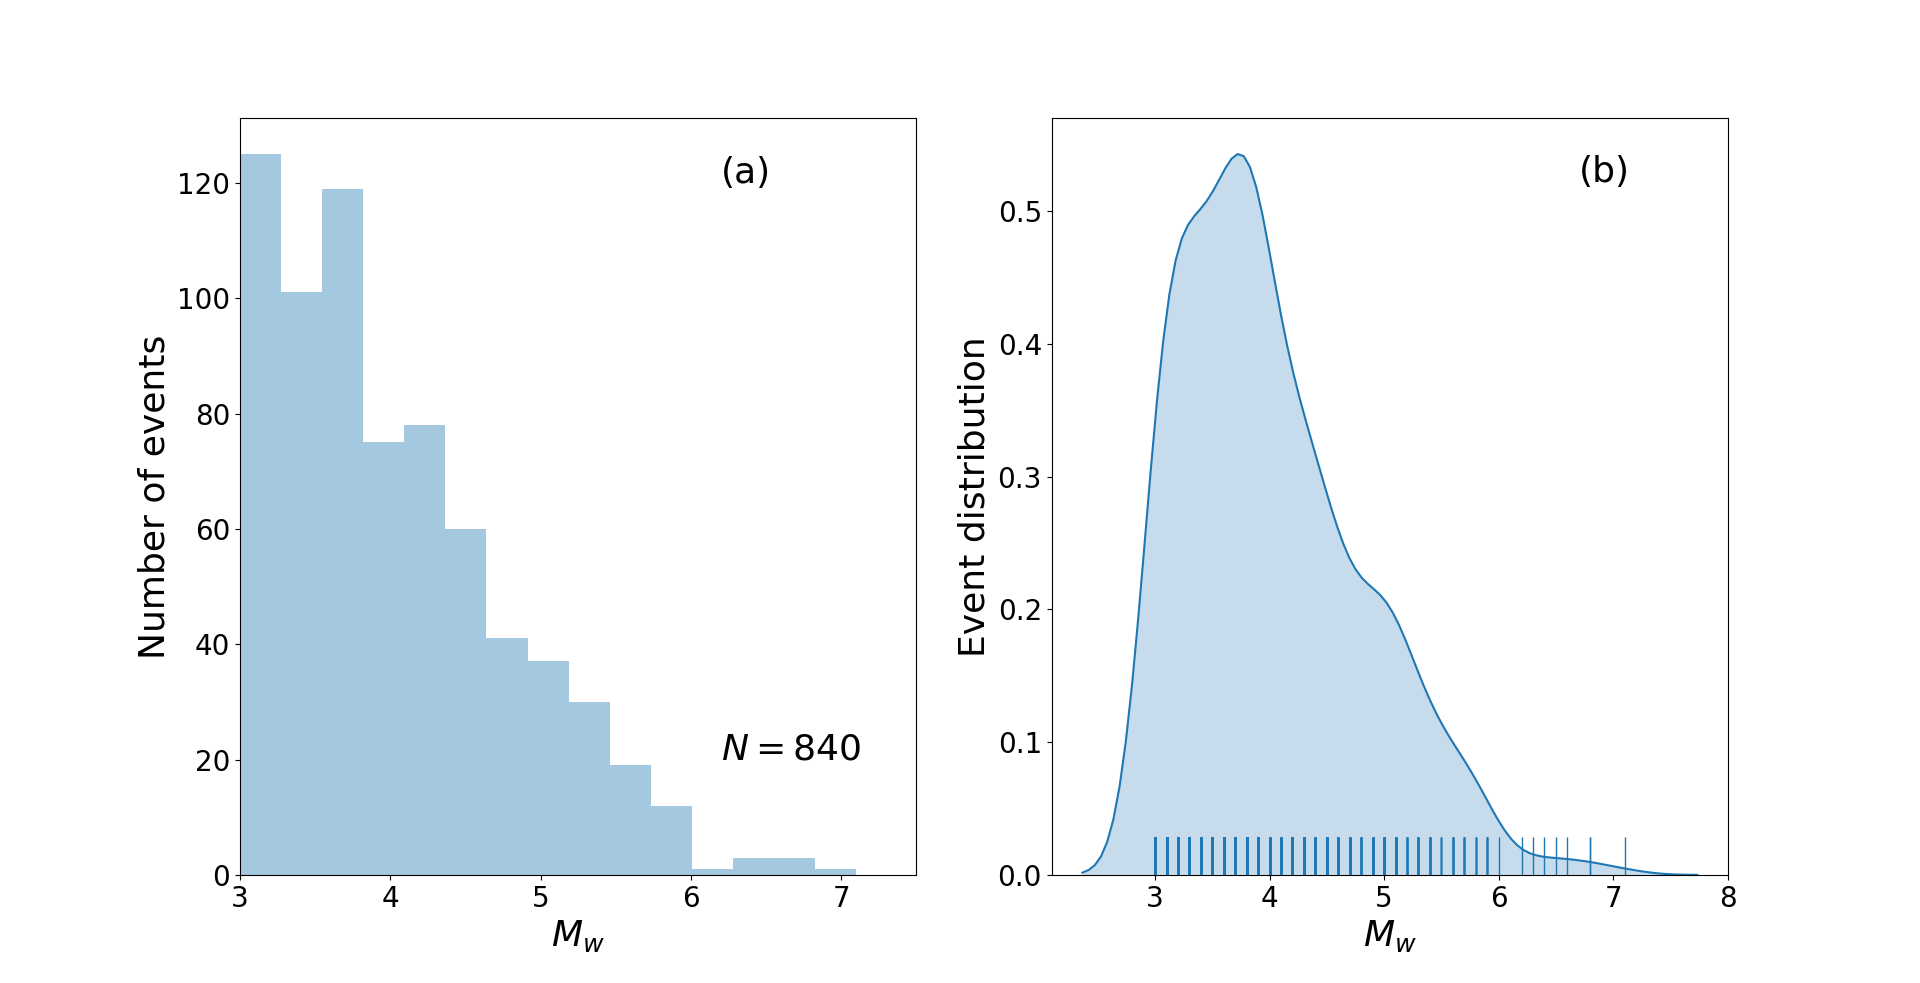
\includegraphics[width=\linewidth]{img/Event_distribution.png}  %插入的图,包括JPG,PNG,PDF,EPS等,放在源文件目录下
	\caption{数据集中地震单条记录的震级分布。横轴为单条记录的震级$\mathbf{M}_{\mathbf{w}}$。\\
(a)图中纵轴为该震级的事件记录数目。(b)图中纵轴为单条记录震级大小分布的概率密度}  %图片的名称
	\label{fig:mcmthesis-logo}   %标签,用作引用
\end{figure}
\indent 图4.3(a)显示了以单一记录为视角的不同震级记录数目的分布。虽然一次地震事件中对于大地震的台站记录数量多于小地震,这使得不同级别地震发生频率上不均衡导致数据不均衡的问题得到一定程度上的缓解,但震级分布总体来看仍然不够均匀,小地震记录条数远远多于大地震。客观上大地震释放的能量巨大,如若不能良好处置则会给人们正常生活生产带来了严重破坏和致命打击,所以大地震往往是紧急预警系统中容错率较低的部分,人们并不希望地震预警系统对于来临大地震没有正确的响应。但从数据量的角度来看大地震出现频率低,可供机器学习模型学习的信息量少,这不利于模型采集到关于如何预估大型地震的规则,给模型的训练带来较大的困扰。\\
\indent 对于类别不均衡,现有的技术大体上有三类做法(周志华, 2016):第一类是对训练集里的正类样本(大地震事件)进行过采样,即通过增加正列数量使得在训练集中、反列样本(大地震事件、小地震事件)数量差距变小。第二类与第一类方法相反,采取对负样本欠采样的方式平衡有偏分布类别。第三类方法为直接对原训练集进行学习,但对训练好的模型评判阈值进行平移,改变评判标准。采取第二种欠采样的方式会丢失很多反例,使得训练集数据量变少,在训练数据有限的情况下并不适用。第三类方法更多的应用于分类问题,不同于我们所设计回归问题。综上我们采取在训练集中对大地震数据过采样再加一定噪音的方法增广正例样本,以此处理数据分布不平衡问题。将原始的如图4.3(a)分布修正为图4.3(b),一定程度上缓解分布不均带来的训练问题。\\
\begin{figure}[!h]%%图
	\centering  %插入的图片居中表示
	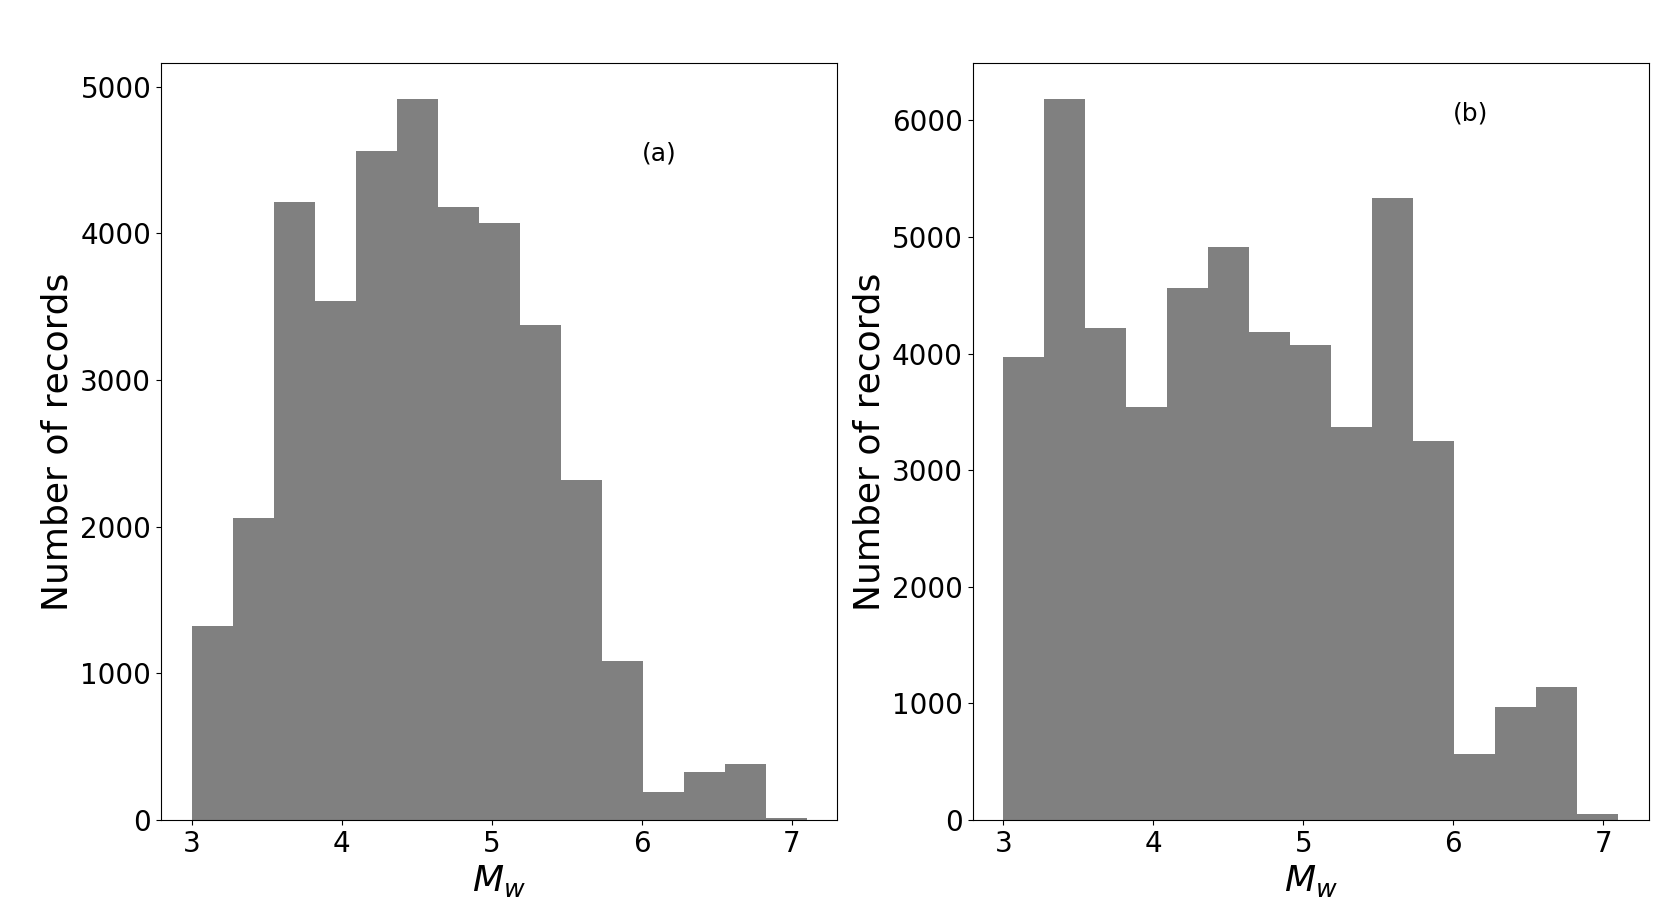
\includegraphics[width=\linewidth]{img/event_dist.png}  %插入的图,包括JPG,PNG,PDF,EPS等,放在源文件目录下
	\caption{数据集中地震记录的震级分布。横轴为震级$\mathbf{M}_{\mathbf{w}}$,纵轴为该震级的台站记录数目。\\
(a) 原始分布;(b) 调整后分布}  %图片的名称
	\label{fig:mcmthesis-logo}   %标签,用作引用
\end{figure}
\section{机器学习类模型与传统模型的比较}
\subsection{NN震级预估模型的效果评估与比较}
\indent 训练曲线如图4.4所示,图中两条图线分别代表了训练集和交叉验证集的均方根误差(RMSE)随着训练步数的变化。NN模型在经过大约15000个步训练步长后,达到此模型结构下的最佳权值状态。超过15000个训练步长后后虽然训练数据集级上模型表现持续变好,但在交叉检验数据集上RMSE停止减小并开始增大,说明模型已经进入第三章所描述的过拟合状态,此时再增加训练轮数只会让模型更加过拟合震级预估能力变得更差。故当完成15000个训练步长时,NN模型触发提前停止条件(Early Stopping),在此训练步数上停止训练并存储此时的模型最佳权值。\\
\begin{figure}[!h]%%图
	\centering  %插入的图片居中表示
	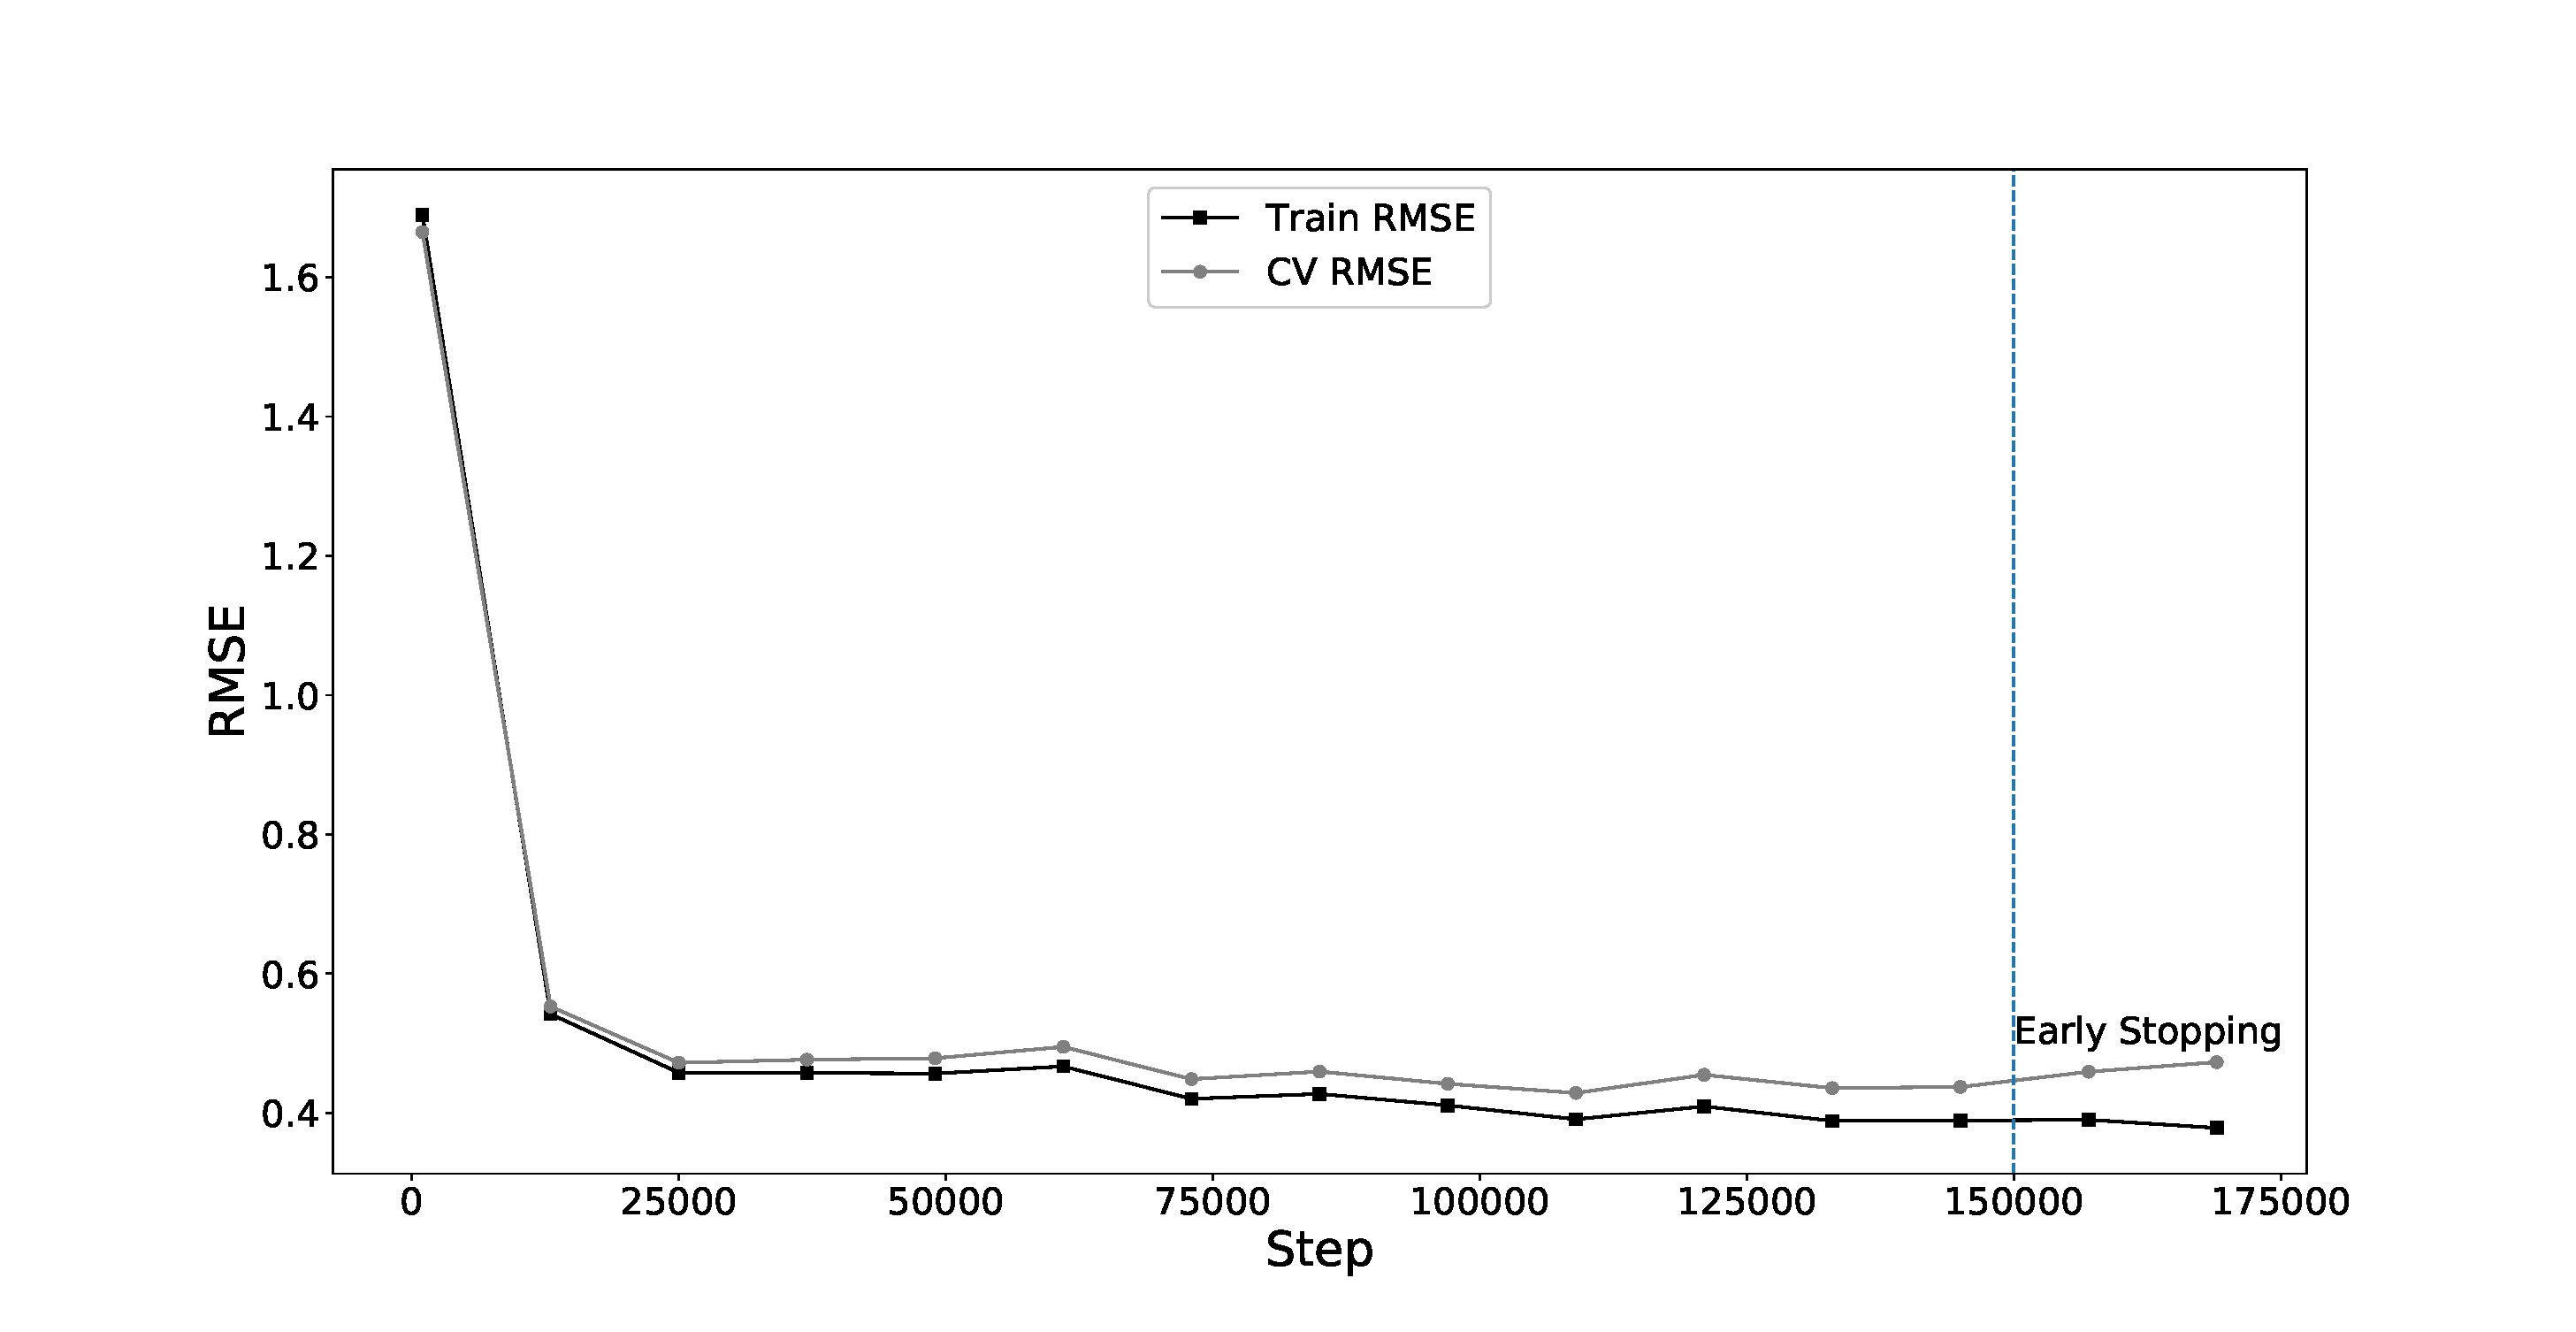
\includegraphics[width=\linewidth]{img/6.eps}  %插入的图,包括JPG,PNG,PDF,EPS等,放在源文件目录下
	\caption{NN模型训练曲线。横轴为训练步数,纵轴为均方根误差(RMSE)。}  %图片的名称
	\label{fig:mcmthesis-logo}   %标签,用作引用
\end{figure}
\indent 在图4.5和4.6中我们还原Kanamori (2008)的$\tau_{\mathrm{c}}$方法(以下简称为“K方法”),并使其与NN模型在同样的测试数据集上相比较。图4.5(a) K方法的结果中的实线为拟合$\tau_{\mathrm{c}}$和$\mathrm{M}_{\mathrm{w}}$的线性关系,实线上下两条虚线代表了一个平均标准差的范围。值得注意的是在Kanamori (2008)中一共使用了来自3个地区共54个事件的集合对$\tau_{\mathrm{c}}$和$\mathrm{M}_{\mathrm{w}}$的线性拟合。每个事件的$\tau_{\mathrm{c}}$值都定义为离震中最近的4个台站$\tau_{\mathrm{c}}$的平均值。这与本文定义略有出入,本文中$\tau_{\mathrm{c}}$值定义为距离震中100km内的所有台站的平均值。\\
\indent 同时K方法中没有进行数据集的分割,其中线性回归模型所使用的训练集和测试集都为同一数据集,即先使用全54个地震事件进行回归模型训练,然后又在这54个事件上进行误差计算。这使得K方法在模型评估效果上存在一定的隐患。在本文的研究实验中所有方法的效果评估都严格按照第3章中所叙述的数据集分割方式进行。\\
\indent 如图4.5所示当NN模型与和K方法考察相同震级范围,都研究震级大于4级的事件区间并以地震事件震级预估误差作为评判。图中的小正方形为多台站联合预估震级的平均结果,而方框上下的延长线为该事件的一个标准差的置信区间。结果显示出NN模型和K方法对于单一地震事件在测试集上的方均根误差别为0.29和0.59。相比于K模型体现出性能明显优势,NN模型预估震级误差更小约为K方法的一半。直观来看在图4.5中NN模型的(a)图相比于K模型的(b)图斜率更大,意味着对于同一特征NN模型有着更强的分辨率。\\
\begin{figure}[!h]%%图
	\centering  %插入的图片居中表示
	\includegraphics[width=\linewidth]{img/7.eps}  %插入的图,包括JPG,PNG,PDF,EPS等,放在源文件目录下
	\caption{震级预估效果对比(最低截至震级为4级)。横轴为真实震级。\\
(a) 采用Kanamori et al. (2008)方法的结果,纵轴为K方法的$\log \left(\tau_{\mathrm{c}}\right)$;\\(b) NN模型的结果,纵轴为机器学习模型给出的预估震级}  %图片的名称
	\label{fig:mcmthesis-logo}   %标签,用作引用
\end{figure}
\indent 如果把研究范围的最小震级限制拓展至3级,按照图4.5的方法得到图4.6所示的结果。将3级至4级地震事件加入到考察范围内后,NN模型和K方法的预估能力都有明显下降。两方法的方均根误差分别升至0.51和1.06,这意味着两类模型对于一定程度的低级别地震震级的预估能力劣于中等级别的地震。\\
\begin{figure}[!h]%%图
	\centering  %插入的图片居中表示
	\includegraphics[width=\linewidth]{img/8.eps}  %插入的图,包括JPG,PNG,PDF,EPS等,放在源文件目录下
	\caption{震级预估效果对比(最低截至震级为3级)。横纵坐标同图4.5。\\
(a) 采用Kanamori et al. (2008)方法的结果;\\(b) NN模型的结果;}  %图片的名称
	\label{fig:mcmthesis-logo}   %标签,用作引用
\end{figure}
\indent 图4.7两子图展示了NN方法和K方法对于不同震级的地震记录,只使用单一台站三分量信息的情况下进行预估的误差情况。整体而言在各个震级上K方法预估的表现虽然稳定但误差均大于NN方法。对所有地震的单台站预估平均误差中,NN方法效果最差误差最大出现在7级以上地震约为1.6级,K方法效果最好误差最小出现在6级地震但平均误差仍有1.1级。\\
\indent K方法中单台站的预测误差大小随着震级增加而略微减小。可能造成这种现象的原因,首先,震级越大其台站接收到的数据信噪比越大,各种噪音对震级预估的影响就越小。其次,如图4.8中所示随着地震事件震级的增大其被记录到的台站数越多,这种特征使得大型地震相对较小地震有更多数据记录。再考虑到$\tau_{\mathrm{c}}$方法的工作流程,最终会使用多台站$\tau_{\mathrm{c}}$的平均值做震级预估时的特征时,自然存在台站越多震级估计的越准确。进而在以地震事件为视角做$\tau_{\mathrm{c}}$与$\mathbf{M}_{\mathbf{w}}$线性回归时得到参数能更好应用于较大型地震的震级预估。注意到在图4.8,因6级以上地震发生频率低数据量较少故并没有进行展示。\\
\indent 图4.7(a)为NN方法下不同震级的误差情况,整体分为蓝色和红色两个区域。中间的蓝色区域内单台站预估出的震级误差稳定,而两侧红色区域误差随震级有较大的变化。4.7(b)中规律佐证了在蓝色区域内,从物理本质上较为容易进行震级预估。这里考虑到首先4级至6级的地震事件被台站记录数量已足够多,其次这个区间地震破裂过程时长适中,能在较好被P波初到后3~s的时长数据所估计。另一方面NN震级预估方法为机器学习方法,其模型解释能力很强。但在两侧红色区域仍不能得到满意的预估结果。这从反面一定程度上说明了在两侧红色区域存在客观问题使得震级预估问题本身不易实现。对于左侧红色区域NN模型的表现与K模型相似都展现出随着震级变大效果变好。\\
\indent 因本文对于P波到时采取比较简单的长短周期自动拾取方式,而小震级地震信号强度低使用此种自动拾取方式误差较大。同时根据经验公式(Wells et al. 1994;孙银涛等, 2016)可知小于4级小型地震破裂持续时间较短通常小于1~s,这使得其对P波到时拾取误差更为敏感,稍有P波初到延后判定就会造成信息量严重丢失比例。并且在这一区域地震信号的低信噪比也是影响预估效果的重要因素,低强度的地震信号更易被噪声所淹没。而右端红色高误差区域为大震级地震区域,存在着两个因素制约着预估精度,第一高能量释放的大地震破裂往往持续较长(从Wells et al.(1994)经验公式可知大于6.5级的地震其破裂时间往往大于10~s)难以被P波初到后3s的数据解释,第二这样的大地震出现的频度较低数据量少不利于训练。\\
\begin{figure}[!h]%%图
	\centering  %插入的图片居中表示
	\includegraphics[width=\linewidth]{img/eb.eps}  %插入的图,包括JPG,PNG,PDF,EPS等,放在源文件目录下
	\caption{不同方法在只使用单台站信息下不同震级地震预估的误差情况\\
(a)NN方法对不同震级地震的预估误差。其中两侧红色区域为预估非稳定区域,中间蓝色区域为稳定区域;\\
(b)K方法对不同震级地震的预估误差;}  %图片的名称
	\label{fig:mcmthesis-logo}   %标签,用作引用
\end{figure}
\begin{figure}[!h]%%图
	\centering  %插入的图片居中表示
	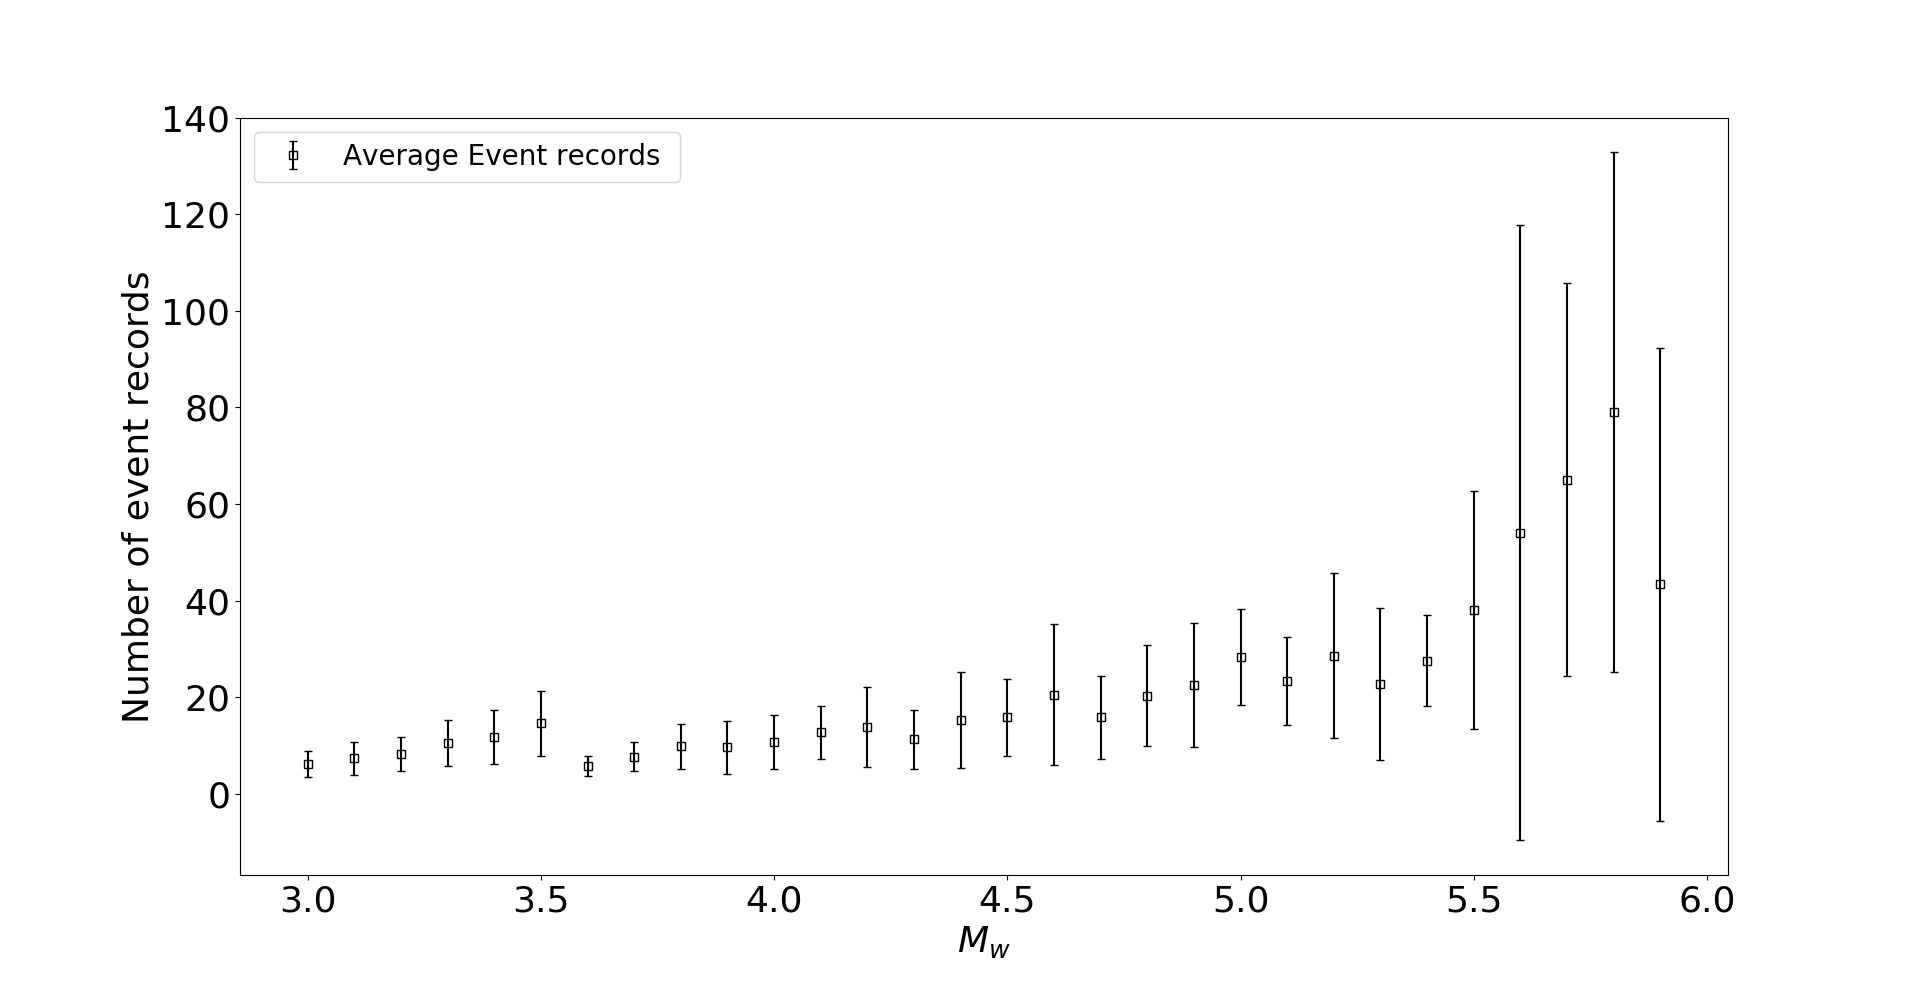
\includegraphics[width=\linewidth]{img/M-N.png}  %插入的图,包括JPG,PNG,PDF,EPS等,放在源文件目录下
	\caption{地震事震级件与其被台站记录数量的关系。横轴为事件震级$\mathbf{M}_{\mathbf{w}}$,纵轴为事件被记录到的数量}  %图片的名称
	\label{fig:mcmthesis-logo}   %标签,用作引用
\end{figure}
\indent 图4.9展示了K方法与NN方法以地震事件为视角震级预估的稳定性情况,图4的两个子图是在设置不同最低截至震级下预估误差方差的分布。可以看出在两种情形下,NN模型预估震级误差的总方差都更小展现出稳定的表现。并且从震级预估的方差分布特点来看,NN模型在两种最低截至震级情形下都展现出左移且高峰度的特点。综合来看,NN模型的稳定性优于Kanamori(2008)的$\tau_{\mathrm{c}}$方法。\\
\begin{figure}[!h]%%图
	\centering  %插入的图片居中表示
	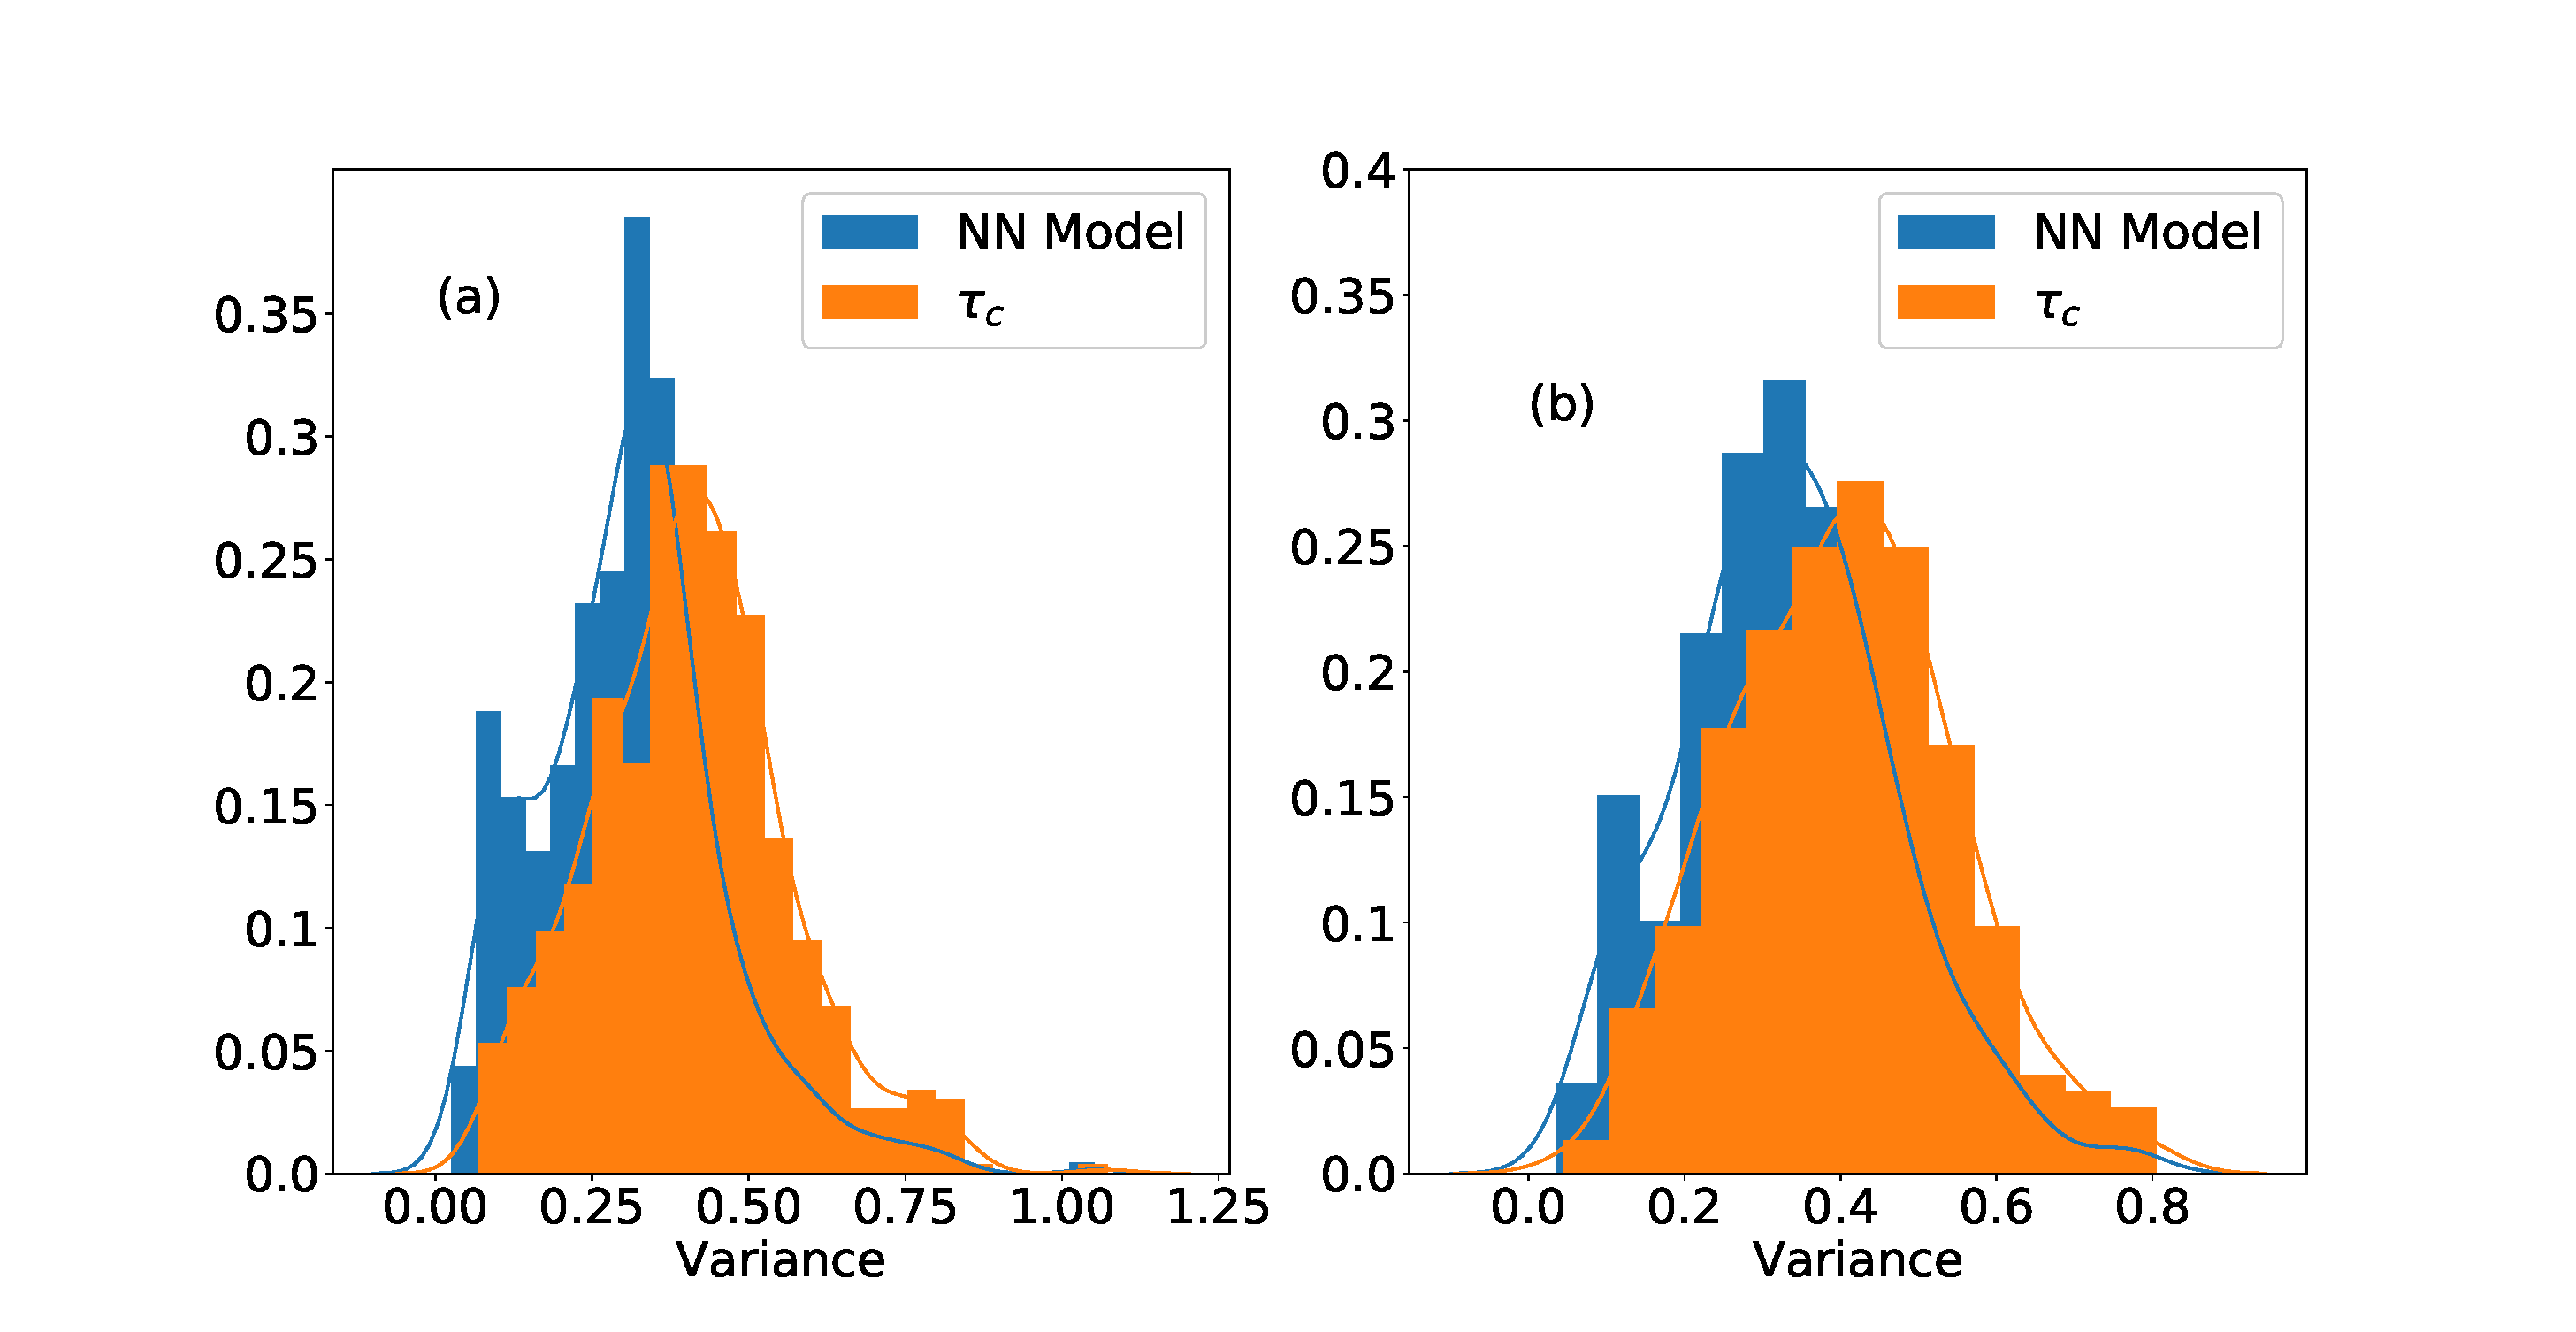
\includegraphics[width=\linewidth]{img/9.eps}  %插入的图,包括JPG,PNG,PDF,EPS等,放在源文件目录下
	\caption{单一事件预估方差分布。横轴为方差大小,纵轴为该方差的密度。\\
(a) 截至震级为4级K方法与NN模型方差分布;\\
(b) 截至震级为3级K方法与NN模型方差分布;\\}  %图片的名称
	\label{fig:mcmthesis-logo}   %标签,用作引用
\end{figure}
\subsection{CNN震级预估模型的效果评估与比较}
\indent 按照3.3.2节中所设计的CNN震级预估模型搭建并完成了相应深度学习神经网络。由于计算机性能限制,本模型只使用了全数据集50\%的数据量进行模型训练与评估。将训练完成的模型在预设的验证集进行效果评估,其结果如图4.10和图4.11所示,可以发现在只使用一半数据量的情况下CNN模型已经展现出超过NN模型的性能。\\
\indent 图4.10显示了对于不同震级的地震记录,在只使用单一台站信息的情况下进行预估的误差情况。在图中存在三种颜色区域,其中两侧的红色仍为震级预估不稳定区域。4级到6级的蓝色区域为稳定区域与NN模型表现相当,3.3级到4级的绿色区域为在NN模型下不稳定变为稳定的区域。因数据量不足和在物理原理上预估可行性的原因,CNN模型在大于6级的区域仍然体现出不够准确的表现。在绿色区域因为CNN模型自身优秀的表达能力和信息量更为充分的输入,使其已部分摆脱原来因小震级地震数据信噪比低带来的预估不准确问题。\\
\indent 图4.11为CNN模型震级预估的具体效果。在最低截至震级为3级情况下方均根误差为0.42优于NN模型结果,在最低截至震级为4级情况下方均根误差为0.29。这与CNN模型对图4.10中绿色小震级区间(3.3级至4级)预估效果改善的分析一致。\\
\begin{figure}[!h]%%图
	\centering  %插入的图片居中表示
	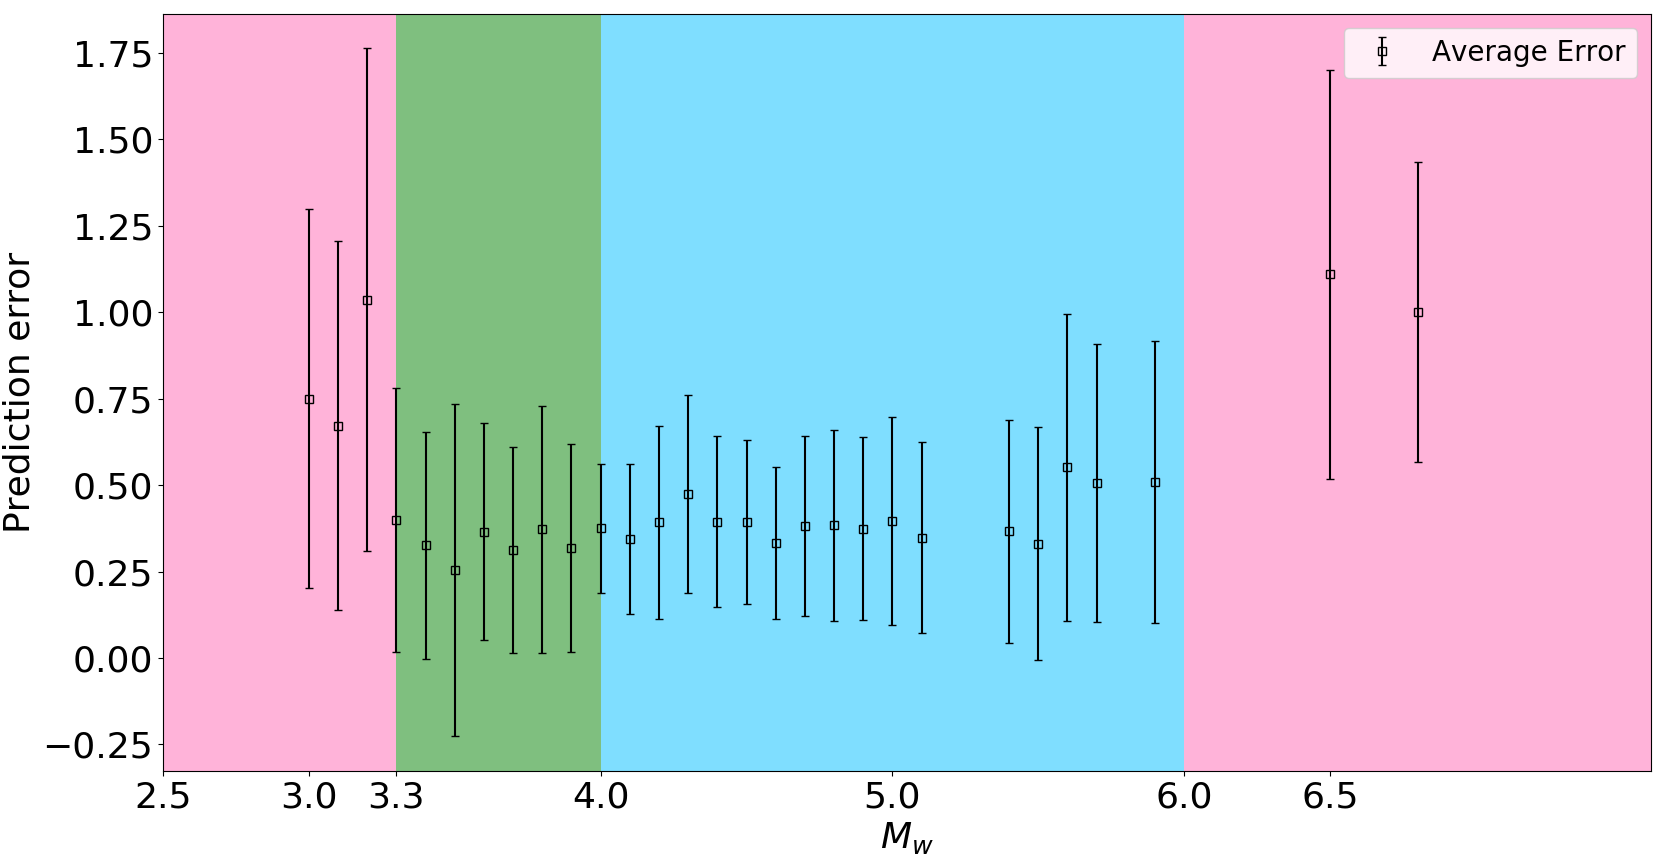
\includegraphics[width=\linewidth]{img/eb1_cnn.jpg}  %插入的图,包括JPG,PNG,PDF,EPS等,放在源文件目录下
	\caption{CNN震级预估模型使用单一台站记录下的误差分布}  %图片的名称
	\label{fig:mcmthesis-logo}   %标签,用作引用
\end{figure}
\begin{figure}[!h]%%图
	\centering  %插入的图片居中表示
	\includegraphics[width=\linewidth]{img/CNN-PRE.eps}  %插入的图,包括JPG,PNG,PDF,EPS等,放在源文件目录下
	\caption{CNN震级预估模型效果图\\
(a)最低震级为3级;(b)最低震级为4级}  %图片的名称
	\label{fig:mcmthesis-logo}   %标签,用作引用
\end{figure}

\subsection{机器学习模型处理低信噪比的效果}
\indent 现实生活中当一次特大地震主震结束后,往往会伴随许多危害巨大的余震出现。虽然这些余震震级相对于主震来说都是较小的,但因建筑物、矿区等各种设施在主震来临时其结构已经遭受一定程度上的破坏,余震的发生往往会进一步破坏本来已经处于危险状况的设施结构,引发进一步的人员伤亡、加剧生产资料损毁,并且有还可能引发其他各种的次生灾害。因此余震震级的紧急预估具有十分重要的研究意义。\\
\indent 传统震级预估方法在面对余震记录时并不能够准备的给出震级预估,低信噪比数据使传统方法在一定程度上趋于无效。而本文中所涉及的两类机器学习类震级预估方法,在处理低信噪比数据是都有着优秀的表现,其中CNN模型表现最优。在初步的研究中我们采用向真实台站数据添加不同幅值的高斯噪声以模拟大地震后分布在尾波中的余震。同时参考John(2018)关于地震记录的信噪比设定为(4.1)、(4.2)式,其中$A_{s}$和$A_{n}$分别为信号和噪音的强度表示,SNR(Signal Noise Ratio)为信噪比。
\begin{equation}
\mathrm{SNR}=10 \log _{10}\left[\left(\frac{A_{\text {s}}}{A_{\text {n}}}\right)^{2}\right]
\end{equation}
\begin{equation}
A_{\text { s }}=\left(\sum_{c=1}^{3} \sum_{t=1}^{300} d_{c, t}^{2}\right)^{1 / 2}
\end{equation}
\indent 不同信噪比的情形下K模型和CNN模型如表4.1所示。因在现实中较大型台站地震的低信噪比数据不太符合现有台站数据质量,故文中若定义信噪比为1则是指使得4级以下地震信噪比基本全部小于1。在这种处理下,当数据集信噪比下降至10时,K模型就出现了严重的震级预估能力下降,若将信噪比下降至1时K模型已经基本完全丧失了对震级的预估能力。相比之下,CNN模型在面对仅是因为加入正态分布白噪声而降低信噪比的数据时,其震级预估能力的基本没有明显下降,CNN模型展现出良好的预估能力。\\
\begin{table}[!h]
\setlength{\abovecaptionskip}{4pt}
\setlength{\belowcaptionskip}{4pt}
\caption{两种方法在不同信噪比下震级预估表现(最低震级为3级)}
\centering 
\begin{tabular}{|c|c|c|} 
\hline 
\diagbox{~~~SNR~~~}{~~RMSE~~}{~~~模型~~~}&~~~~~~CNN模型~~~~~~&~~~~~~Kanamori模型~~~~~~\\ %添加斜线表头
\hline $+\infty$&0.44&1.06\\ 
\hline 10&0.45&1.8\\ 
\hline 1&0.64&2.5\\ 
\hline \end{tabular} 
\end{table} 
\indent 图4.11与图4.12具体展示了CNN模型在面对低信噪比数据时表现情况。可以看出分别以3级和4级作为截止频率时CNN模型的方均根误差为别升至0.64和0.37,误差整体有所上升但仍处于可以接受的范围。预估效果进行横向比较,CNN模型在面对有噪音的数据集时其误差仍然低于处理不添加噪音的K模型。其结果表明CNN模型强大的表达能力使神经网络获得滤除噪音的能力。而K模型抗噪能力较差并没任何滤波能力,添加任何噪音进入原始信号都会使得K模型给出更高的震级预估。\\
\begin{figure}[!h]%%图
	\centering  %插入的图片居中表示
	\includegraphics[width=\linewidth]{img/no_CNN_PRE.eps}  %插入的图,包括JPG,PNG,PDF,EPS等,放在源文件目录下
	\caption{CNN震级预估模型效果图\\
(a)最低震级为3级;(b)最低震级为4级}  %图片的名称
	\label{fig:mcmthesis-logo}   %标签,用作引用
\end{figure}
\begin{figure}[!h]%%图
	\centering  %插入的图片居中表示
	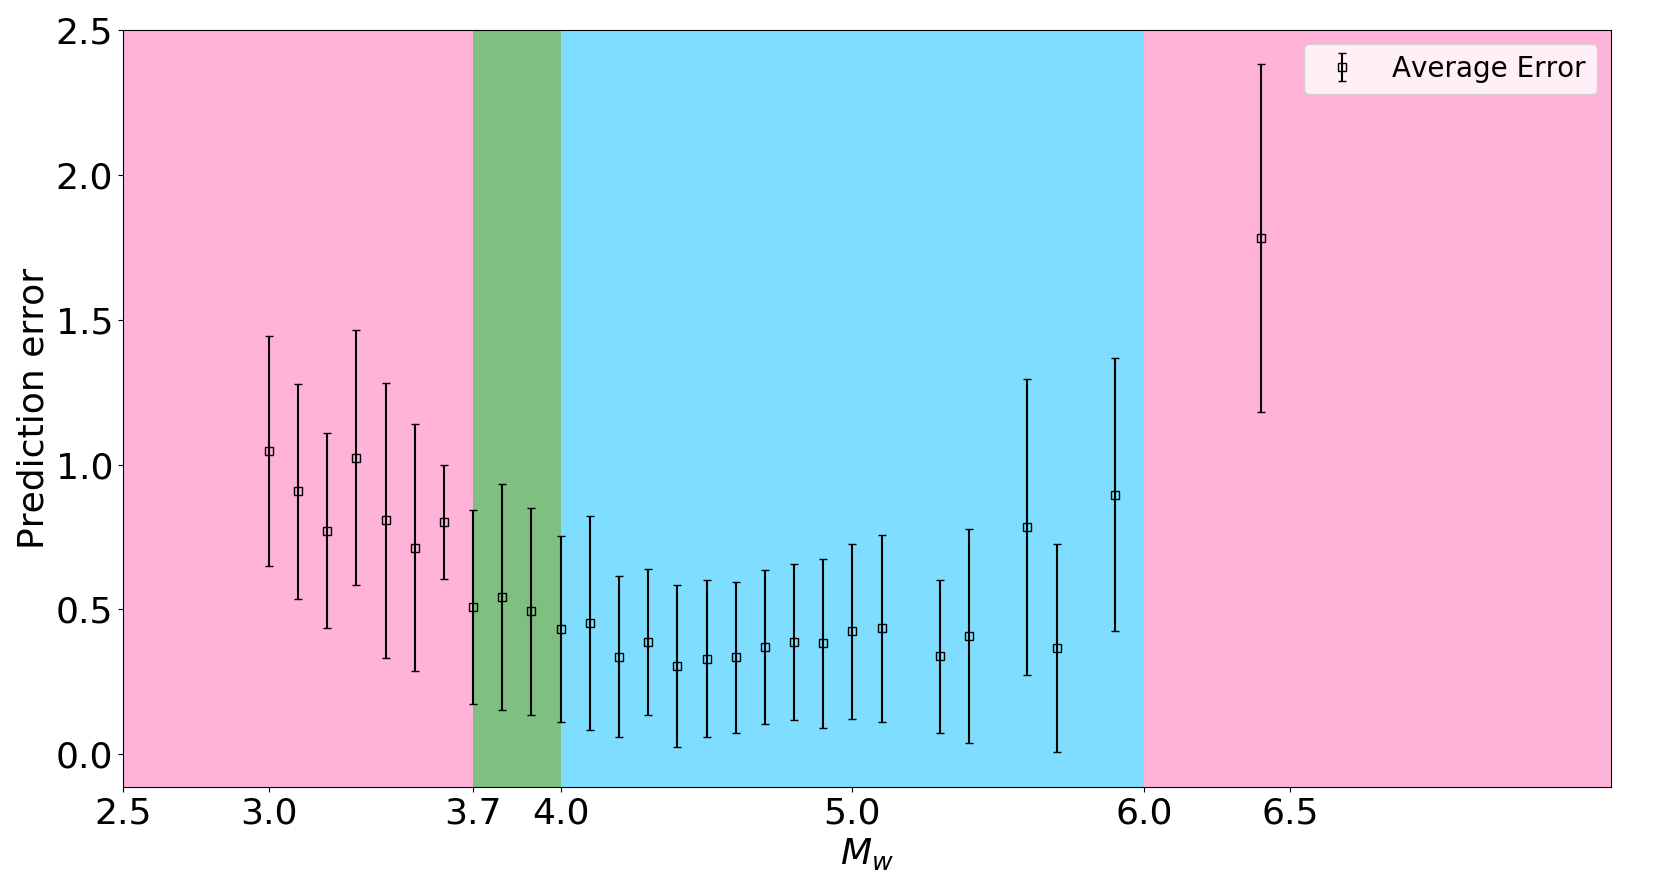
\includegraphics[width=\linewidth]{img/eb1_no_cnn.jpg}  %插入的图,包括JPG,PNG,PDF,EPS等,放在源文件目录下
	\caption{CNN震级预估模型在信噪比约等于1的数据集上,只使用单台站信息下不同震级地震预估的误差情况}  %图片的名称
	\label{fig:mcmthesis-logo}   %标签,用作引用
\end{figure}
\indent 如图4.13和图4.14所示向原始数据集中加入高斯噪音后,CNN模型绿色预估稳定区域变窄其左端向右移动,这与前文中对造成红色不稳定区可能原因的猜测一致。高斯噪音使得原本就为低信噪比的地震级区域信噪比继续降低预估难度加大,还体现为图4.14中3级至4级区域内代表有噪音的数据集黄线整体在代表原始数据的蓝线之上。而右侧的4级至6级区域因本身信号强度足够,故并未受到噪音的影响。\\
\begin{figure}[!h]%%图
	\centering  %插入的图片居中表示
	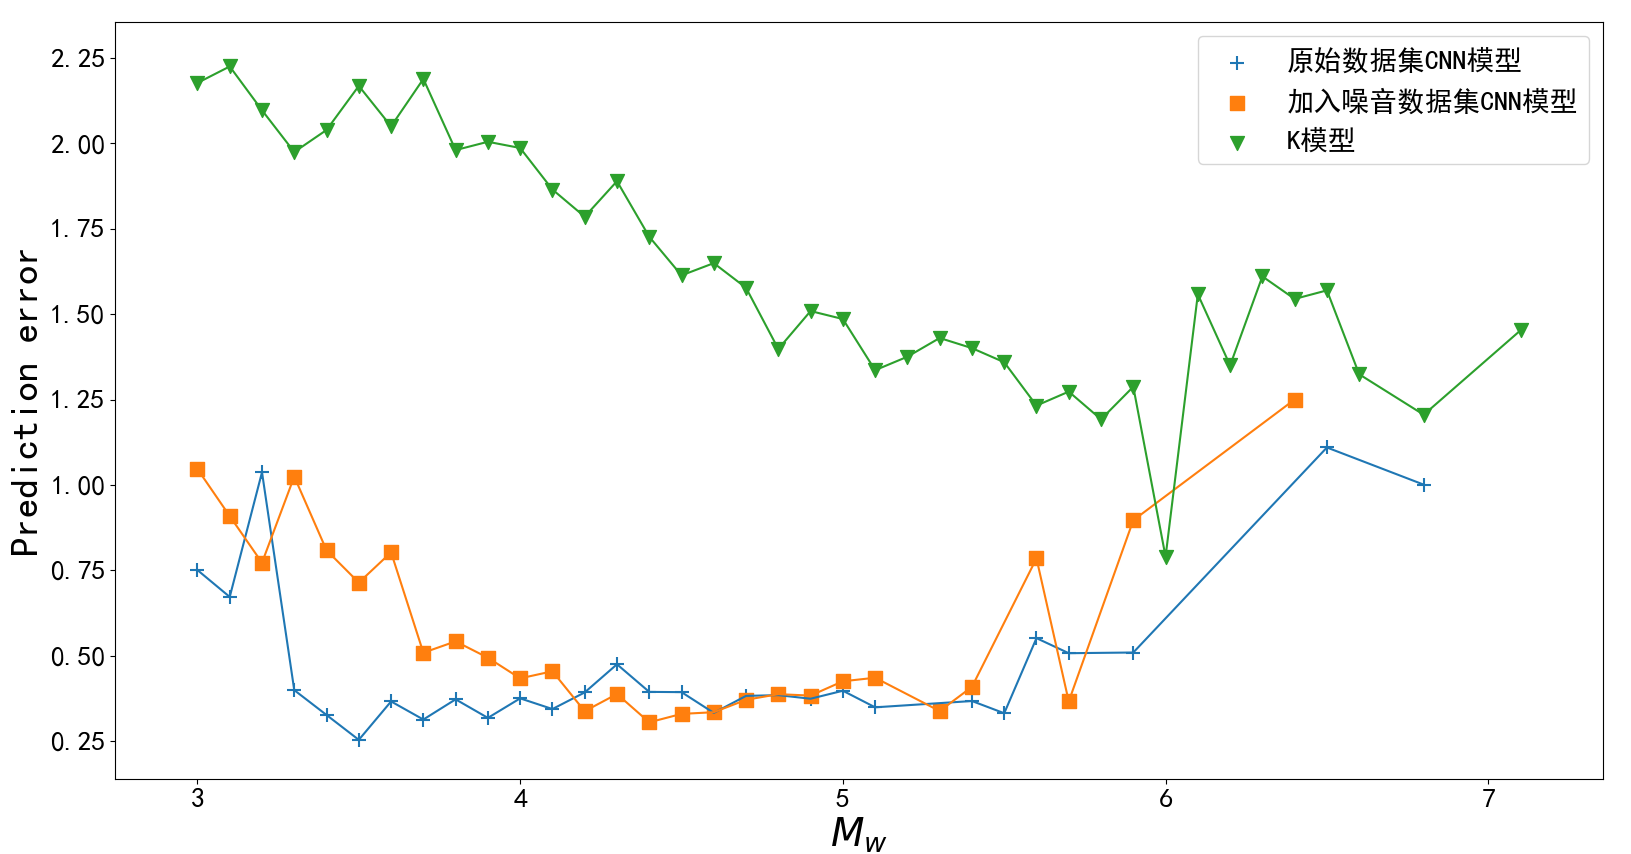
\includegraphics[width=\linewidth]{img/model_comparison.jpg}  %插入的图,包括JPG,PNG,PDF,EPS等,放在源文件目录下
	\caption{两种模型在不同信噪比下不同震级地震预估的误差情况}  %图片的名称
	\label{fig:mcmthesis-logo}   %标签,用作引用
\end{figure}




